% ---- Acronyms ----
\newacronym{amr}{AMR}{Autonomous Mobile Robot}
\newacronym{api}{API}{Application Programming Interface}
\newacronym{csa}{CSA}{Canadian Standards Association}
\newacronym{gui}{GUI}{Graphical User Interface}
\newacronym{imu}{IMU}{Inertial Measurement Unit}
\newacronym{ir}{IR}{Infrared}
\newacronym{iso}{ISO}{International Organization for Standardization}
\newacronym{lidar}{LiDAR}{Light Detection and Ranging}
\newacronym{mbps}{Mbps}{Megabits per second}
\newacronym{msha}{MSHA}{Mine Safety \& Health Administration}
\newacronym{ppe}{PPE}{Personal Protective Equipment}
\newacronym{rc}{RC}{Remote Control}
\newacronym{ui}{UI}{User Interface}

% ---- Definitions ----
\newglossaryentry{anomalies}{
  name=Anomalies,
  description={Deviations in the map because of a mining collapse}
}
\newglossaryentry{payload}{
  name=Payload,
  description={The part of the vehicle’s load where objects of need are derived, e.g., oxygen tanks, medical supplies, and water tanks}
}
\newglossaryentry{persons}{
  name={Persons in Need},
  description={Miners trapped in the mine}
}
\newglossaryentry{scalability}{
  name=Scalability,
  description={Feature to add a team-designed autonomous robot to the existing fleet}
}
\newglossaryentry{operations_hub}{
  name={Operations Hub},
  description={Source of the mesh network}
}
\newglossaryentry{foundational}{
  name={Foundational Goals},
  description={Functional goals fundamental to the completion of the autonomous mobile robot}
}
\newglossaryentry{applied}{
  name={Applied Goals},
  description={Non-functional requirements based on Red Chris Mine and industry}
}
\newglossaryentry{innovative}{
  name={Innovative Goals},
  description={Goals which focus on research and fulfilling a gap that the team identified in the industry with a potential solution}
}
\newglossaryentry{safe_mode}{
  name={Safe Mode},
  description={Mode the autonomous robot enters, which shuts down motors, causing the robot to stop moving}
}
\newglossaryentry{ibex}{
  name={Ibex Platform},
  description={Existing platform, which will be used as the chassis for the autonomous robot}
}
\newglossaryentry{features}{
  name={Features},
  description={Discrete, identifiable functionalities of the \gls{amr} and \gls{fleet} used to track technical progress and ensure traceability}
}
\newglossaryentry{fleet}{
  name={The Fleet},
  description={The complete group of robots, comprising the \gls{amr} and the two \gls{rc} robots}
}

\section{Executive Summary}
\label{sec:executive_summary}

The Search \& Support Fleet Robotics project focuses on post-disaster relief. A disaster is unpredictable; the aftermath creates an unknown environment, which lacks reliable infrastructure. A collapsed mine may disconnect a centralized computer network. The robot fleet will be able to traverse an unknown environment, relay information and share responsibilities using a mesh network to optimize the search and support process. \gls{fleet} will comprise of one payload-carrying \gls{amr} and two manually operated support robots. The \gls{amr} will be built on the \gls{ibex} robot chassis, while the support robots will utilize \gls{rc} car platforms. 

\gls{fleet} will be capable of detecting \gls{anomalies} in the environment, searching for \gls{persons}, supplying support (water, oxygen and medical kit) to those individuals, and relaying information to the \gls{operations_hub}, see \autoref{fig:fleet_visual_representation}. 

The project's goals define the functional and non-functional requirements that must be met. The metrics of the goals define quantitative baselines that prove that the objectives have been achieved. The numerical goals are based on a case study of a mining collapse at the Red Chris mine, as well as initial calculations and industry baselines. At the Red Chris mine, three workers were trapped underground for 60 hours, without communication with the surface for the majority of that time.

The goals of the project include the following, and are thoroughly defined in \nameref{sec:requirements}, with all assumptions and constraints defined in \nameref{sec:assumptions_constraints}.

\begin{enumerate}
    \item The Fleet shall \textbf{detect \gls{anomalies}} in the mine.
    \item The Fleet shall \textbf{locate \gls{persons}} in need.
    \item The Fleet shall \textbf{carry a \gls{payload} to persons in need} of life support.
    \item The Fleet shall \textbf{establish communication} with persons in need and relay telemetry for monitoring the state of the mine.
    \item The Fleet shall \textbf{be scalable}.
\end{enumerate}

The overall goal of this project is to create a safer, faster, and more effective emergency response system. To achieve this goal, the team will develop a unified system that integrates robotics, sensing, and networking to advance disaster relief operations in the mining industry. This results in both a functional prototype and a framework for autonomous rescue fleets.

\begin{figure}[H]
    \centering
    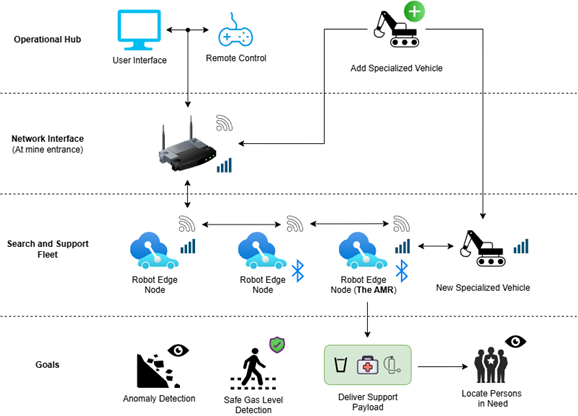
\includegraphics[width=0.9\textwidth]{images/project_visual_representation.png}
    \caption{Search \& Support Fleet Robotics visual representation}
    \label{fig:fleet_visual_representation}
\end{figure}
